\documentclass[tikz]{standalone}
\usepackage{pgfplots}
\pgfplotsset{compat=1.15}
\usepackage{mathrsfs}
\usetikzlibrary{arrows,calc}
\usepackage{tkz-euclide}

\pagestyle{empty}

\definecolor{AngleClr}{rgb}{0,0.39215686274509803,0}
\definecolor{ShapeClr}{rgb}{0.6,0.2,0}
\definecolor{BlueClr}{RGB}{5,81,163}

\begin{document}

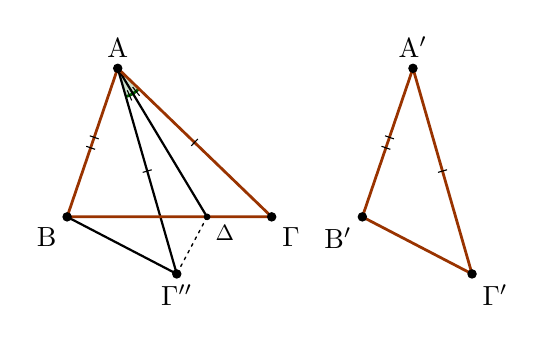
\begin{tikzpicture}[scale=.75]
\tkzSetUpLine[line width=1pt,color=black]
\tkzSetUpPoint[fill=black]

\tkzDefPoints{0/0/C1,5/0/C2}
\tkzDefShiftPoint[C1](120:1.75){A}
\tkzDefShiftPoint[C1](-150:2){B}
\tkzDefShiftPoint[C1](-30:2){C}

% \tkzDefPointOnLine[pos=0.7](A,B)\tkzGetPoint{M}




\tkzDefPointsBy[rotation=center A angle -30](C){M}
\tkzDefPointsBy[rotation=center A angle -15](C){DD}

\tkzDefPointsBy[translation=from C1 to C2](A,B,M){AA,BB,CC}


\tkzInterLL(A,DD)(B,C) \tkzGetPoint{D}


\tkzFillPolygon[fill=white](A,B,C)

\tkzFillPolygon[fill=white](AA,BB,CC)

%\tkzFillAngles[fill=AngleClr,size=.4,fill opacity=0.2](B,A,C BB,AA,CC)
%\tkzMarkAngles[line width=1pt,color=AngleClr,size=.4](B,A,C BB,AA,CC)

%\tkzFillAngles[fill=AngleClr,size=.4,fill opacity=0.2](C,B,A CC,BB,AA)
%\tkzMarkAngles[mark=||,mksize=2,line width=1pt,color=AngleClr,size=.4](C,B,A CC,BB,AA)

\tkzFillAngles[fill=AngleClr,size=.5,fill opacity=0.2](D,A,C M,A,D)
\tkzMarkAngles[mark=|,mksize=2,size=.5,line width=1pt,color=AngleClr](D,A,C M,A,D)

\tkzDrawSegments[line width=0.5pt,color=black,dashed,dash pattern=on 1pt off 1.75pt](D,M)
\tkzDrawSegments[line width=0.8pt](B,M A,D A,M)

\tkzDrawPolygon[color=ShapeClr](A,B,C)
\tkzDrawPolygon[color=ShapeClr](AA,BB,CC)

\tkzDrawPoints[size=3](A,B,C,AA,BB,CC,M)
\tkzDrawPoints[size=2](D)

\tkzLabelPoint[above](A){$\rm A$}
\tkzLabelPoint[below left](B){$\rm B$}
\tkzLabelPoint[below right](C){$\rm \Gamma$}
\tkzLabelPoint[below right,scale=0.8](D){$\rm \Delta$}
\tkzLabelPoint[below](M){$\rm \Gamma''$}
\tkzLabelPoint[above](AA){$\rm A'$}
\tkzLabelPoint[below left](BB){$\rm B'$}
\tkzLabelPoint[below right](CC){$\rm \Gamma'$}

\tkzMarkSegments[mark=||,size=1.7](A,B AA,BB)
\tkzMarkSegments[mark=|,size=1.7](A,C AA,CC A,M)

\end{tikzpicture}

\end{document}
